% Generated 2020-01-10 14:19:52 -0800
\subsection{Conditions} \label{model:Conditions}

\begin{figure}[ht]
  \centering
    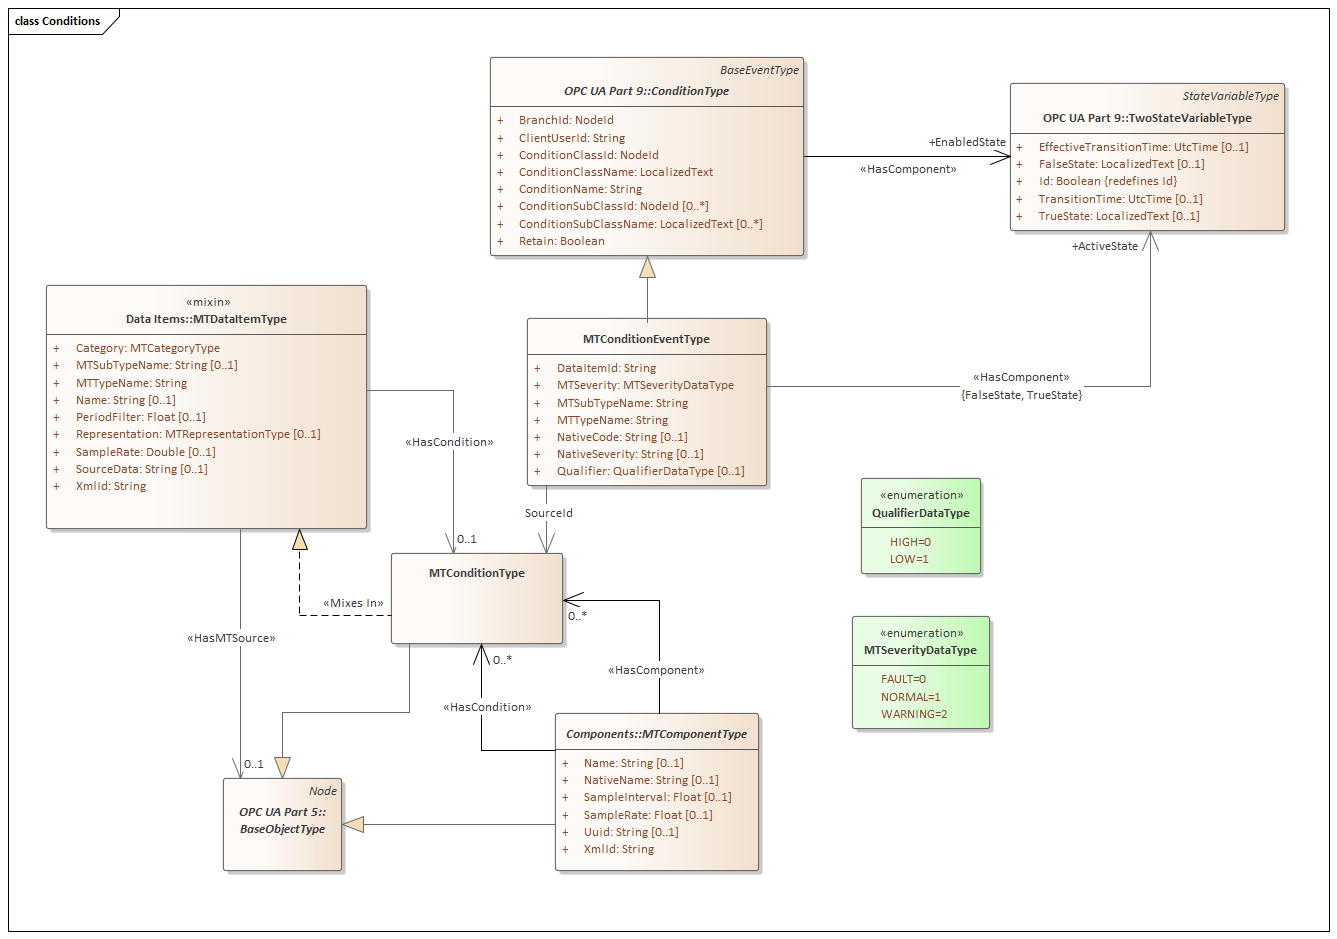
\includegraphics[width=1.0\textwidth]{./diagrams/types/Conditions.png}
  \caption{Conditions Diagram}
  \label{fig:Conditions}
\end{figure}

\FloatBarrier


\input ./type-sections/Conditions.tex

\subsubsection{Defintion of \texttt{ MTConditionEventType}}
  \label{type:MTConditionEventType}

\FloatBarrier

The condition type is a derived from the UA \uamodel{ContitionType}. When the \mtmodel{Warning} or \mtmodel{Fault} state occurs, an \mtuatype{MTConditionEventType} \uamodel{Event} is created and with the \mtmodel{ActiveState} set to \uamodel{True} and \uamodel{Retain} set to \uamodel{True}.
The severity is used to represent the MTConnect condition states of Warning and Fault with the values of 500 and 1000 respectively. 

A new \uamodel{NodeId} will be created for every unique instance of the MTConnect \mtmodel{Condition} reported.  When the \mtmodel{Condition} goes back to Normal, the \mtmodel{ActiveState} is set  to \uamodel{False} and \uamodel{Retain} is also set to \uamodel{False} with the \uamodel{NodeId} of the associated \mtmodel{Condition}. If multiple MTConnect \mtmodel{Condition}s have been cleared at the same time, all currently active \mtuatype{MTConditionEventType} \uamodel{Event}s will need to be created as inactive.

The \mtuatype{MTConditionEventType} must set the \uamodel{BaseEvent} \uamodel{SourceNode} to the related \mtuatype{MTConditionType} that represents the meta-data for this Condition.

The \mtuatype{MTConditionEventType} will never be instantiated in the \uaterm{AddressSpace} as an \uamodel{Object}. 


\begin{table}[ht]
\centering 
  \caption{\texttt{MTConditionEventType} Definition}
  \label{table:MTConditionEventType}
\fontsize{9pt}{11pt}\selectfont
\tabulinesep=3pt
\begin{tabu} to 6in {|X[-1.35]|X[-0.7]|X[-1.75]|X[-1.5]|X[-1]|X[-0.7]|} \everyrow{\hline}
\hline
\rowfont\bfseries {Attribute} & \multicolumn{5}{|l|}{Value} \\
\tabucline[1.5pt]{}
BrowseName & \multicolumn{5}{|l|}{MTConditionEventType} \\
IsAbstract & \multicolumn{5}{|l|}{False} \\
\tabucline[1.5pt]{}
\rowfont \bfseries References & NodeClass & BrowseName & DataType & Type\-Definition & {Modeling\-Rule} \\
\multicolumn{6}{|l|}{Subtype of ConditionType (See \cite{UAPart9} Documentation)} \\
Has\-Property & Variable & Active\-State & Localized\-Text & Property\-Type & Mandatory \\
Has\-Property & Variable & Data\-Item\-Id & String & Property\-Type & Mandatory \\
Has\-Property & Variable & MT\-Severity & MT\-Severity\-Data\-Type & Property\-Type & Mandatory \\
Has\-Property & Variable & MT\-Sub\-Type\-Name & String & Property\-Type & Mandatory \\
Has\-Property & Variable & MT\-Type\-Name & String & Property\-Type & Mandatory \\
Has\-Property & Variable & Native\-Code & String & Property\-Type & Optional \\
Has\-Property & Variable & Native\-Severity & String & Property\-Type & Optional \\
Has\-Property & Variable & Qualifier & Qualifier\-Data\-Type & Property\-Type & Optional \\
\end{tabu}
\end{table} 


\FloatBarrier
\paragraph{Referenced Properties and Objects}

\begin{itemize}
\item \texttt{DataItemId : String:}  The identifier attribute of the dataitem that represents the originally measured value of the data referenced by this data item.

\item \textbf{Allowable Values} for \texttt{MTSeverityDataType}
\FloatBarrier




\begin{table}[ht]
\centering 
  \caption{\texttt{MTSeverityDataType} Enumeration}
  \label{enum:MTSeverityDataType}
\tabulinesep=3pt
\begin{tabu} to 6in {|l|r|X|} \everyrow{\hline}
\hline
\rowfont\bfseries {Name} & {Index} & {Description} \\
\tabucline[1.5pt]{}
\texttt{FAULT} & \texttt{0} & Fault value for a condition element. \\
\texttt{NORMAL} & \texttt{1} & Normal value for a condition element. \\
\texttt{WARNING} & \texttt{2} & Warning value for a condition element. \\
\end{tabu}
\end{table} 
\FloatBarrier
\item \texttt{NativeCode : String:} When instantiated in the address space this will represent the \mtmodel{NativeCode} of the last
\uaterm{Event} that was received. When the ActiveState becomes False and becomes 
inactive, then the \mtmodel{NativeCode} will be cleared. The native code (usually an alpha-numeric value) generated by the controller of a piece of equipment or the element.

\item \texttt{NativeSeverity : String:} When instantiated in the address space this will represent the \mtmodel{NativeSeverity} of the last
\uaterm{Event} that was received. When the ActiveState becomes False and becomes 
inactive, then the \mtmodel{NativeSeverity} will be cleared. If the piece of equipment designates a severity level to a fault, nativeseverity reports that severity information to a client software application. 

\item \texttt{Qualifier : QualifierDataType:}  qualifier provides additional information regarding a fault state associated with the measured value of a process variable.

\item \textbf{Allowable Values} for \texttt{QualifierDataType}
\FloatBarrier



\begin{table}[ht]
\centering 
  \caption{\texttt{QualifierDataType} Enumeration}
  \label{enum:QualifierDataType}
\tabulinesep=3pt
\begin{tabu} to 6in {|l|r|X|} \everyrow{\hline}
\hline
\rowfont\bfseries {Name} & {Index} & {Description} \\
\tabucline[1.5pt]{}
\texttt{HIGH} & \texttt{0} & High qualifier value for a condition element. \\
\texttt{LOW} & \texttt{1} & Low qualifier value for a condition element. \\
\end{tabu}
\end{table} 
\FloatBarrier
\item \texttt{SourceName : MTConditionType:} The \uamodel{SourceName} is mapped to the \uamodel{BrowseName} of the \mtuatype{MTConditionType}.

\item \texttt{SourceNode : MTConditionType:} The \uamodel{SourceNode} is mapped to the \uamodel{NodeId} of the \mtuatype{MTConditionType}.

\end{itemize}
\FloatBarrier
\subsubsection{Defintion of \texttt{ MTConditionType}}
  \label{type:MTConditionType}

\FloatBarrier

An \mtmodel{MTConditionType} instance will be created for event MTConnect \gls{MTDataItem} with a 
\gls{category} of \mtmodel{CONDITION}. 

The \gls{BrowseName} of the condition uses the same naming convention as the  MTConnect
\gls{MTDataItem} types with \gls{MTCondition} appended as a suffix. For example the 
condition with \gls{type} of \mtmodel{TEMPERATURE} will have the browse name of 
\mtmodel{TemperatureCondition} as opposed to the \mtuatype{MTSampleType} of \mtmodel{Temperature}.

An XML element which provides the information and data reported from a piece of equipment for those dataitem elements defined with a category attribute of condition category in the mtconnectdevices document.

\begin{table}[ht]
\centering 
  \caption{\texttt{MTConditionType} Definition}
  \label{table:MTConditionType}
\fontsize{9pt}{11pt}\selectfont
\tabulinesep=3pt
\begin{tabu} to 6in {|X[-1.35]|X[-0.7]|X[-1.75]|X[-1.5]|X[-1]|X[-0.7]|} \everyrow{\hline}
\hline
\rowfont\bfseries {Attribute} & \multicolumn{5}{|l|}{Value} \\
\tabucline[1.5pt]{}
BrowseName & \multicolumn{5}{|l|}{MTConditionType} \\
IsAbstract & \multicolumn{5}{|l|}{False} \\
\tabucline[1.5pt]{}
\rowfont \bfseries References & NodeClass & BrowseName & DataType & Type\-Definition & {Modeling\-Rule} \\
\multicolumn{6}{|l|}{Subtype of BaseObjectType (See \cite{UAPart5} Documentation)} \\
Has\-Property & Variable & Category & MT\-Category\-Type & Property\-Type & Mandatory \\
Has\-Property & Variable & MT\-Sub\-Type\-Name & String & Property\-Type & Optional \\
Has\-Property & Variable & MT\-Type\-Name & String & Property\-Type & Mandatory \\
Has\-Property & Variable & Name & String & Property\-Type & Optional \\
Has\-Property & Variable & Period\-Filter & Float & Property\-Type & Optional \\
Has\-Property & Variable & Representation & MT\-Representation\-Type & Property\-Type & Optional \\
Has\-Property & Variable & Sample\-Rate & Double & Property\-Type & Optional \\
Has\-Property & Variable & Source\-Data & String & Property\-Type & Optional \\
Has\-Property & Variable & Xml\-Id & String & Property\-Type & Mandatory \\
Has\-MT\-Source & Object & <Base\-Object> & \multicolumn{2}{l|}{BaseObjectType} & Optional \\
Has\-MT\-Composition & Object & <MT\-Composition> & \multicolumn{2}{l|}{MTCompositionType} & Optional \\
Has\-MT\-Sub\-Class\-Type & Object & <MT\-Data\-Item\-Sub\-Class> & \multicolumn{2}{l|}{MTDataItemSubClassType} & Optional \\
Has\-Condition & Object & <MT\-Condition> & \multicolumn{2}{l|}{MTConditionType} & Optional \\
Has\-Component & Object & Constraints & \multicolumn{2}{l|}{MTConstraintType} & Optional \\
Has\-MT\-Class\-Type & Object & <MT\-Data\-Item\-Class> & \multicolumn{2}{l|}{MTDataItemClassType} & Mandatory \\
\end{tabu}
\end{table} 


\paragraph{Dependencies and Relationships}

\begin{itemize}
\item Mixes in \texttt{MTDataItemType}, see See section \ref{type:MTDataItemType}
\end{itemize}
\FloatBarrier
